
\documentclass{book}

\usepackage[obeyspaces]{url} % Force the url{} to respect spaces.

\usepackage{
  array,          % vertically-centered tabular cells
  calculator,     % arithmetic operators
  draftwatermark, % diagonal DRAFT watermark
  enumerate,      % enumerate with letter labels
  fancyhdr,       % custom chapter headings
  fullpage,       % reasonable margins
  graphicx,       % inline graphics (ABET logo, assist.org screenshots)
  hyperref,       % hotlinks
  ifthen,         % if statements
  makeidx,        % index
  multirow,       % table elements may span columns/rows
  tcolorbox,      % background colors in Tip sidebars
  tikz,           % used to draw prerequisite trees and flowcharts
  times,          % font choice
}


\newcommand{\IsDraft}{0} % assign nonzero for DRAFT watermark, zero for no watermark

\newcommand{\UsePDFCourseGraph}{1} % assign nonzero for PDF course graph, zero for original LaTeX course graph 

\usetikzlibrary{patterns} % for time-critical course hatching
    
% Don't say "Chapter 3", just "3"
\renewcommand{\chaptername}{}

% do not indent paragraphs horizontally
\setlength{\parindent}{0pt}

% blank line between paragraphs
\setlength{\parskip}{12pt}

% draft watermark
\ifnum \IsDraft=0
  \SetWatermarkText{}
\else
  \SetWatermarkText{DRAFT}
  \SetWatermarkColor[gray]{0.9}
\fi

% tip sidebar
\newenvironment{tip}{
  \tcolorbox \begin{tabular}{m{.5in} m{5.25in}}
    \Large{TIP} &
}{
  \end{tabular} \endtcolorbox
}

% name of our campus, so this is consistent everywhere (i.e. "CSUF",
% not "CSU Fullerton")
\newcommand{\CampusName}{CSUF}

% names of tracks
\newcommand{\CtTrackName}{Custom (CT)}
\newcommand{\IeTrackName}{Internet and Enterprise Computing (IE)}
\newcommand{\IsTrackName}{Cybersecurity (IS)}
\newcommand{\MgTrackName}{Multimedia and Digital Games (MG)}
\newcommand{\ScTrackName}{Scientific Computing (SC)}
\newcommand{\SeTrackName}{Software Engineering (SE)}

% track index entries
\newcommand{\MakeTrackIndexCommand}[2]{
  \newcommand{#1}{\index{track!#2}}
}
\MakeTrackIndexCommand{\CtTrackIndex}{\CtTrackName}
\MakeTrackIndexCommand{\IeTrackIndex}{\IeTrackName}
\MakeTrackIndexCommand{\IsTrackIndex}{\IsTrackName}
\MakeTrackIndexCommand{\MgTrackIndex}{\MgTrackName}
\MakeTrackIndexCommand{\ScTrackIndex}{\ScTrackName}
\MakeTrackIndexCommand{\SeTrackIndex}{\SeTrackName}

% \shrunkurl{name}
%
% Produces a visible and clickable link to the shrunk URL with the
% given name.
%
% Example:
%   \shrunkurl{cs}
% Expands to a clickable link that displays as
%   csuf-cpsc.appspot.com/cs
\newcommand{\shrunkurl}[1]{\url{http://csufcs.com/#1}}

% prerequisite tree figure

% \GenericTreeCourse{tikz style}{tikz identifier}{X-coord}{Y-coord}{CPSC/MATH/ENGL}{course number}
% draw a low-level course node
\newcommand{\GenericTreeCourse}[5]{
  \node [#1] (#3) at (#4, #5) {#2 #3};
}

% \TimeCriticalTreeCourse{tikz identifier}{X-coord}{Y-coord}{CPSC/MATH/ENGL}{course number}
% draw a time-critical course node
\newcommand{\TimeCriticalTreeCourse}[4]{
  \GenericTreeCourse{draw, rounded corners, pattern=north west lines, pattern color=black!30!white}{#1}{#2}{#3}{#4}
}

% \TreeCourse{tikz identifier}{X-coord}{Y-coord}{CPSC/MATH/ENGL}{course number}
% draw a non-time-critical course node
\newcommand{\TreeCourse}[4]{
  \GenericTreeCourse{draw, rounded corners}{#1}{#2}{#3}{#4}
}

% \StraightPrereq{subject course identifier}{course identifier it depends upon}
% straight-line prerequisite edge
\newcommand{\StraightPrereq}[2]{
  \draw [thick, ->] (#2) -- (#1);
}

% \BentPrereq{subject course identifier}{course identifier it depends upon}
% bent (curved) prerequisite edge
\newcommand{\BentPrereq}[3]{
  \draw [thick, ->] (#2) edge [#3] node {} (#1);
}

% \Coreq{subject course identifier}{course identifier it depends upon}
% straight corequisite edge
\newcommand{\Coreq}[2]{
  \draw [thick, dashed] (#1) -- (#2);
}

% \IntroTree{X-coord}
% draw nodes for the 120-121-131 intro tree; used for both the major
% and minor figures
\newcommand{\IntroTree}[1]{
  \TimeCriticalTreeCourse{CPSC}{120}{#1}{0}
  \TimeCriticalTreeCourse{CPSC}{121}{#1}{-1}
  \TimeCriticalTreeCourse{CPSC}{131}{#1}{-2}
  \StraightPrereq{121}{120}
  \StraightPrereq{131}{121}
}

% \MajorTree
% draw the entire major prerequisite tree. This is a macro since it
% appears twice.
\newcommand{\MajorTree}{
  \ifnum \UsePDFCourseGraph=0
    % there should be exactly 23 courses in the diagram
    \begin{center}
      \begin{tikzpicture}

        % MATH 150A-150B-338 column
        \TimeCriticalTreeCourse{MATH}{150A}{0}{0}
        \TimeCriticalTreeCourse{MATH}{150B}{0}{-1}
        \TimeCriticalTreeCourse{MATH}{338}{0}{-4}
        \StraightPrereq{150B}{150A}
        \StraightPrereq{338}{150B}

        % MATH 270A-270B column
        \TimeCriticalTreeCourse{MATH}{270A}{3}{0}
        \TimeCriticalTreeCourse{MATH}{270B}{3}{-1}
        \StraightPrereq{270B}{270A}

        % CPSC 120-121-131-254-EPP-323 column
        \IntroTree{9}
        \TimeCriticalTreeCourse{CPSC}{254}{9}{-3}
        \TimeCriticalTreeCourse{CPSC}{301}{9}{-4}
        \TreeCourse{CPSC}{323}{9}{-5}
        \StraightPrereq{254}{131}
        \StraightPrereq{301}{254}
        \StraightPrereq{323}{301}

        % 335, 481 under 270
        \TimeCriticalTreeCourse{CPSC}{335}{3}{-5}
        \TimeCriticalTreeCourse{CPSC}{481}{3}{-6}
        \StraightPrereq{335}{270B} \StraightPrereq{335}{338} \StraightPrereq{335}{301}
        \StraightPrereq{481}{335}
  
        % 131 follow-ons
        \TreeCourse{CPSC}{240}{5}{-3}
        \TreeCourse{CPSC}{223}{7}{-3}
        \TreeCourse{CPSC}{332}{11}{-3}
        \TreeCourse{CPSC}{311}{14}{-3}
        \StraightPrereq{240}{131} \BentPrereq{240}{270A}{bend left=30}
        \StraightPrereq{223}{131}
        \StraightPrereq{332}{131}

        % 440 below 240
        \TreeCourse{CPSC}{440}{5}{-6}
        \StraightPrereq{440}{240}
  
        % 351, 471 under 254
        \TreeCourse{CPSC}{351}{12}{-4}
        \TreeCourse{CPSC}{471}{12}{-6}
        \StraightPrereq{351}{254}
        \StraightPrereq{471}{351}

        % 362, ENGL 101 aligned with 311
        \TreeCourse{ENGL}{101}{14}{0}
        \TreeCourse{CPSC}{362}{14}{-5}
        \StraightPrereq{311}{101} \BentPrereq{311}{131}{bend left=15}
        \StraightPrereq{362}{301} \StraightPrereq{362}{311}

        % 315
        \TreeCourse{CPSC}{315}{15}{-4}
        \StraightPrereq{315}{311}

        % legend
        \node at (12.5, -9) {\underline{Legend}};
  
        \TimeCriticalTreeCourse{time-critical}{course}{10}{-10}
  
        \TreeCourse{}{other course}{10}{-11}
  
        \TreeCourse{}{A}{9}{-12}
        \TreeCourse{}{B}{11}{-13}
        \StraightPrereq{B}{A}
        \node at (12, -12.25) {A is a prerequisite for B};

        % there aren't any corequisites left in the diagram
        %\TreeCourse{}{C}{9}{-14}
        %\TreeCourse{}{D}{11}{-14}
        %\Coreq{C}{D}
        %\node at (14, -14) {C and D are corequisites};
  
      \end{tikzpicture}
    \end{center}
  \else
    \begin{center}
      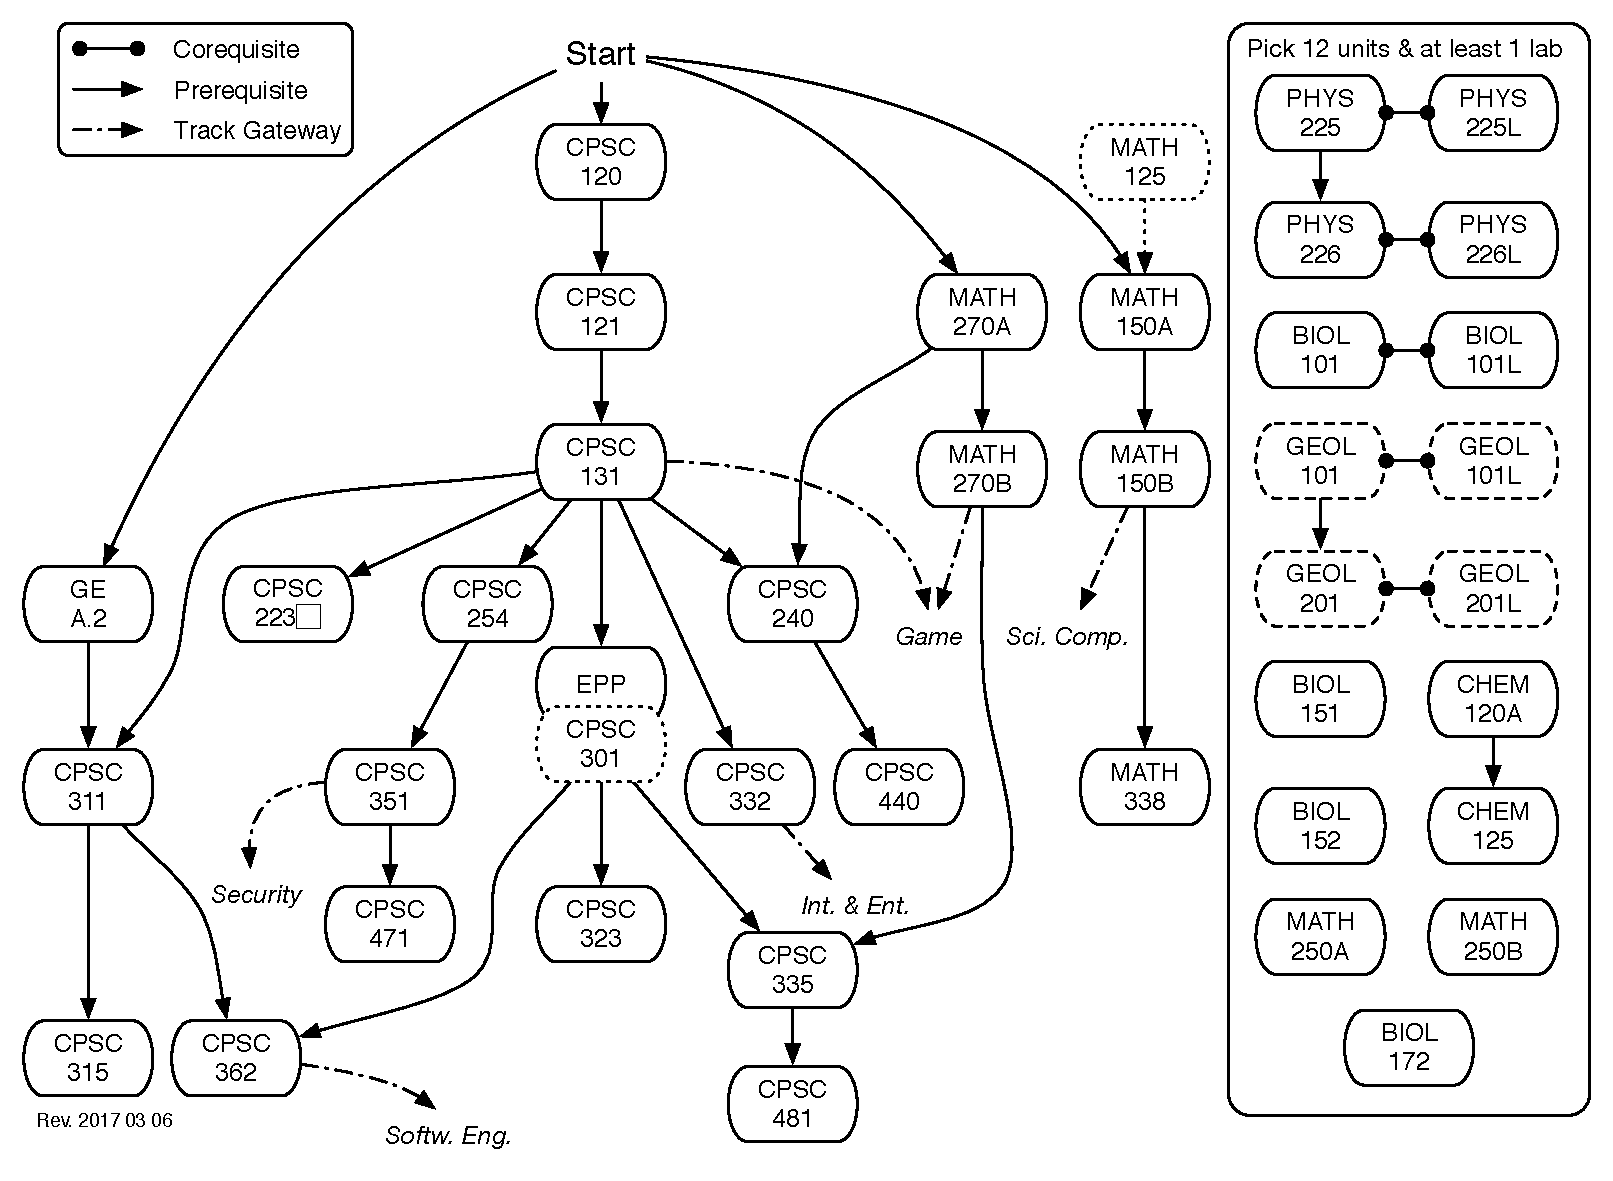
\includegraphics[width=.9\linewidth]{images/cpsc_prerequisites}
    \end{center}
  \fi
}

% \MinorTree
% draw the entire minor prerequisite tree
\newcommand{\MinorTree}{
  \begin{center}
    \begin{tikzpicture}

      \IntroTree{0}

      \TimeCriticalTreeCourse{CPSC}{elective}{0}{-3}
      \StraightPrereq{elective}{131}

      \TreeCourse{GE}{B4}{4}{-2}
      \TreeCourse{CPSC}{313}{4}{-3}
      \StraightPrereq{313}{B4}

    \end{tikzpicture}
  \end{center}
}

% end of prerequisite tree code

%%%%%%%%%%%%%%%%%%%%%%%%%%%%%%%%%%%%%%%%%%%%%%%%%%%%%%%%%%%%%%%%%%%%%%%%%%%%%%%%%%%%%%%%
% flowchart code
%%%%%%%%%%%%%%%%%%%%%%%%%%%%%%%%%%%%%%%%%%%%%%%%%%%%%%%%%%%%%%%%%%%%%%%%%%%%%%%%%%%%%%%%

% rotated 90 degrees clockwise, for landscape mode
\tikzstyle{FlowchartStyle}=[rotate=-90]

% fill colors for course boxes
\newcommand{\CoreColor}{red!30!white}
\newcommand{\MathRequirementColor}{blue!30!white}
\newcommand{\ScienceMathElectiveColor}{green!30!white}
\newcommand{\TrackColor}{red!10!white}
\newcommand{\GeColor}{yellow!30!white}

% these coordinate parameters are kind of a quick and dirty hack
\newcommand{\FlowchartInitialX}{0}
\newcommand{\FlowchartInitialY}{-2}
\newcommand{\FlowchartColumnWidth}{2.8}
\newcommand{\FlowchartYearLabelOffset}{1.4}
\newcommand{\FlowchartRowHeight}{2}
\newcommand{\FlowchartTitleX}{0}
\newcommand{\FlowchartTitleY}{1.5}

% \FlowchartLabel{X-coord}{Y-coord}{text}
% draw a text label
\newcommand{\FlowchartLabel}[3]{
  \node [FlowchartStyle, align=left] at (#1, #2) {#3};
}

% \FlowchartBox{fill color}{label text}{X-coord}{Y-coord}
% draw a flowchart box with an edge and fill color
\newcommand{\FlowchartBox}[4]{
  \node [FlowchartStyle, draw, rectangle, fill=#1, minimum width=1.8, minimum height=1.8, align=left] at (#3, #4) {#2};
}

% \FallSemester{year number, 1 through 4}
% declare the start of a Fall semester
\newcommand{\FallSemester}[1]{
  % compute X-coordinate
  \ifnum #1=1
      % first ever call, initialize \flowX
      \COPY{\FlowchartInitialX}{\flowX}
  \else
      % increment \flowX
      \ADD{\flowX}{\FlowchartColumnWidth}{\flowX}
  \fi

  % reset Y-coordinate
  \COPY{\FlowchartInitialY}{\flowY}

  % Year number label
  \ADD{\flowX}{\FlowchartYearLabelOffset}{\sol}
  \FlowchartLabel{\sol}{0}{Year #1}

  % column header
  \FlowchartLabel{\flowX}{-1}{Fall}
}

% \SpringSemester
% declare the start of a Spring semester
\newcommand{\SpringSemester}{
  \ADD{\flowX}{\FlowchartColumnWidth}{\flowX}
  \COPY{\FlowchartInitialY}{\flowY}

  \FlowchartLabel{\flowX}{-1}{Spring}
}

% \GenericFlowchartCourse{fill color}{label text}
% Add a generic course to the flowchart. Low-level helper for the
% friendlier macros below.
\newcommand{\GenericFlowchartCourse}[2]{
  \FlowchartBox{#1}{#2}{\flowX}{\flowY}
  \SUBTRACT{\flowY}{\FlowchartRowHeight}{\flowY}
}

% Add a course of a specific type and color.
\newcommand{\CoreCourse}[1]{ \GenericFlowchartCourse{\CoreColor}{#1} }
\newcommand{\MathRequirementCourse}[1]{ \GenericFlowchartCourse{\MathRequirementColor}{#1} }
\newcommand{\ScienceMathElectiveCourse}[1]{ \GenericFlowchartCourse{\ScienceMathElectiveColor}{#1} }
\newcommand{\TrackCourse}[1]{ \GenericFlowchartCourse{\TrackColor}{#1} }

\newcommand{\GeCourse}[2]{ \GenericFlowchartCourse{\GeColor}{GE #1 \\ #2} }

% \HarmonizedFlowchart{name}{223 course name}{track1}{track2}...{track5}
\newcommand{\HarmonizedFlowchart}[7]{
  \clearpage
  \begin{tikzpicture}[FlowchartStyle]
    
    % title
    \node [FlowchartStyle, align=left, anchor=west, minimum width=2in] at (\FlowchartTitleX, \FlowchartTitleY) { {\LARGE #1} };

    % lower division
    
    \FallSemester{1}
    \CoreCourse{CPSC 120}
    \MathRequirementCourse{CPSC 270A}
    \MathRequirementCourse{CPSC 150A}
    \GeCourse{A.1}{HCOM 102}
    \GeCourse{A.2}{ENGL 101}
    
    \SpringSemester
    \CoreCourse{CPSC 121}
    \MathRequirementCourse{MATH 270B}
    \MathRequirementCourse{MATH 150B}
    \GeCourse{C.1}{ART 101}
    \GeCourse{C.2}{PHIL 100}
    
    \FallSemester{2}
    \CoreCourse{CPSC 131}
    \ScienceMathElectiveCourse{MATH 250A}
    \GeCourse{C.4}{HIST 110A}
    \GeCourse{D.3}{HIST 170A}
    \GeCourse{D.4}{POSC 100}
    
    \SpringSemester
    \CoreCourse{#2} % 223
    \ScienceMathElectiveCourse{PHYS 225+L}
    \CoreCourse{CPSC 240}
    \CoreCourse{CPSC 254}
    \CoreCourse{CPSC 332}

    % upper division
    \FallSemester{3}
    \CoreCourse{CPSC 351}
    \CoreCourse{CPSC 311}
    \MathRequirementCourse{MATH 338}
    \TrackCourse{#3} % track1

    \SpringSemester
    \CoreCourse{CPSC 335}
    \CoreCourse{CPSC 471}
    \CoreCourse{CPSC 362}
    \ScienceMathElectiveCourse{PHYS 226+L}
    \TrackCourse{#4} % track2

    \FallSemester{4}
    \CoreCourse{CPSC 323}
    \CoreCourse{CPSC 481}
    \GeCourse{D.1}{EGxx 401}
    \GeCourse{C.3 \& Z}{MUS 303}
    \TrackCourse{#5} % track3

    \SpringSemester
    \CoreCourse{CPSC 315}
    \CoreCourse{CPSC 440}
    \TrackCourse{#6} % track4
    \TrackCourse{#7} % track5
    
    % legend at the bottom
    \FlowchartLabel{0}{-12}{Color Legend:}
    \FlowchartBox{\CoreColor}{Core Course}{3}{-12}
    \FlowchartBox{\MathRequirementColor}{Math Req.}{6}{-12}
    \FlowchartBox{\ScienceMathElectiveColor}{Science/Math Elect.}{9}{-12}
    \FlowchartBox{\TrackColor}{Track Course}{12}{-12}
    \FlowchartBox{\GeColor}{Gen. Ed.}{15}{-12}
    
  \end{tikzpicture}
}

% end of flowchart code

% initialize index
\makeindex

\begin{document}

\title{Undergraduate Handbook \\ 2016-2017 Edition}
\author{Department of Computer Science \\ California State University, Fullerton}
\date{Draft: \today}
\maketitle

\newpage
\tableofcontents

\chapter{Introduction}

\section{The Field of Computer Science}
Computer Science is the systematic study of computing systems and computation. The body of knowledge contains the theoretical foundation for understanding computing systems and methods, design methodology, algorithms, and software and hardware tools.

These programs cover a wide range of areas, including:
\begin{itemize}
\item multimedia and digital game technologies,
\item Internet and enterprise computing,
\item wireless and mobile computing,
\item databases and data mining,
\item computer security,
\item software engineering, and
\item computational bioinformatics.
\end{itemize}

Computer Science prepares graduates for rewarding careers in all areas of business, government, education and industry. These organizations, large and small, need computer professionals to address their needs with specific programs and systems. Computer science professionals tackle complicated problems and create computer solutions to solve them, devising new ways to use computers.

\section{The Department}
\label{section:the_department}
The faculty and staff of the Computer Science Department welcome you into our program and sincerely wish you good luck on your journey into higher education, and continued success.

Whenever you have a question about the Department---its policies, its curriculum, its services, your progress, or anything else---feel free to contact us.

\index{contact information}
\begin{tabular}{r p{6in}} % right column in p mode so postal address can have newlines
  Web: & \url{http://fullerton.edu/ecs/cs/} or \shrunkurl{cs} \\ \index{website}
  E-mail: & \href{mailto:csoffice@ecs.fullerton.edu}{\url{csoffice@ecs.fullerton.edu}} \\ \index{e-mail}
  In person: & Room CS-522 \\ \index{department office}
  Telephone: & (657) 278-3700 \\ \index{phone number} \index{telephone number}
  Fax: & (657) 278-7168 \\ \index{fax number}
  Postal mail: & California State University, Fullerton \newline\index{postal address}\index{address}Department of Computer Science \newline
P.O. Box 6870 \newline
Fullerton, CA 92834-6870
\end{tabular}

\section{Accreditation} \index{accreditation}\index{ABET}

The Bachelor of Science in Computer Science degree at \CampusName~is accredited by the Computing Accreditation Commission of ABET (\url{http://www.abet.org}).

\begin{center}
  \fbox{ 
\includegraphics{CAC-CMYK-W.pdf} }
\end{center}

\section{The Programs}

The Department offers the following Undergraduate programs, which are documented in this Handbook:
\begin{enumerate}
\item Bachelor of Science in Computer Science (B.S. CS), and
\item Minor in Computer Science.
\end{enumerate}

The Department also offers Graduate programs, which are documented elsewhere:
\begin{enumerate}
\item Master of Science in Computer Science (M.S. CS),
\item Master of Science in Software Engineering (M.S.E.), and
\item Accelerated Master of Science in Software Engineering (A.M.S.E.).
\end{enumerate}

CS courses are also components of Computer Engineering, Electrical Engineering, and Mathematics programs at \CampusName.

\section{Objectives and Outcomes}
\index{Program Educational Objectives (PEOs)} \index{Program Outcomes}
The Program Educational Objectives and Program Outcomes for the CS B.S. are documented in the University Catalog at \shrunkurl{major}.

\section{Using This Document}

This handbook covers information on how to complete a B.S. or a Minor in Computer Science, and contains information relevant to students pursuing them. If you are pursuing a Masters degree, please refer to the Graduate Handbook instead of this document (\shrunkurl{gradhandbook}).

In order to minimize duplicated information, this document references other documents rather than copying their content. The PDF version of this Handbook presents these references as clickable links.

Some aspects of our programs are complex, and you may find it difficult to choose among alternatives. In those cases, we present our suggested default choice as a tip, as shown below. You are not required to follow these tips, but doing so is often a prudent choice.
\index{tips}
\begin{tip}
When in doubt, heed tips such as this one.
\end{tip}

This document has been formatted so that it may be printed as a booklet. Print double-sided with staples (or other binding) on the left side. The document will look best if printed in color, but it may also be printed in grayscale (a.k.a. semitone).

Prior versions of this document included a \emph{Major Progress Check Sheet.} This is no longer included, since the \emph{Print Degree Planner} link on the CS B.S. page in the University Catalog (\shrunkurl{major}) produces an equivalent checklist form.

\chapter{Sources of Information}

You may find the following sources to be helpful.
\begin{itemize}
\item The University Catalog: \url{http://catalog.fullerton.edu/}
\item Undergraduate Handbook (this document): \shrunkurl{ugradhandbook}
\item Graduate Handbook: \shrunkurl{gradhandbook}
\item Advising:
  \begin{itemize}
    \item CS Department Advising: \shrunkurl{advising}
    \item Center for Academic Support in ECS (CASECS): \shrunkurl{casecs}
    \item Student Success Center: \shrunkurl{ssc}
    \item Academic Advisement Center (GE advising): \url{https://www.fullerton.edu/aac/}
    \end{itemize}
\item Department of Computer Science: \shrunkurl{cs}
\item General Education (GE): \shrunkurl{ge}
\item Course transfer database: \url{http://www.assist.org}
\item Center for Internships \& Community Engagement --- Academic Internships: \shrunkurl{cice}
\item Catalogs of nearby community colleges:
  \begin{itemize}
    \item Cypress College: \url{http://www.cypresscollege.edu/academics/CollegeCatalog.aspx}
    \item Fullerton College: \url{http://www.fullcoll.edu/catalog}
    \item Golden West College: \url{http://www.goldenwestcollege.edu/catalog/}
    \item Irvine Valley College: \url{http://www.ivc.edu/catalog/Pages/catalog2014.aspx}
    \item Orange Coast College: \url{http://www.orangecoastcollege.edu/academics/CourseCatalog/Pages/default.aspx}
    \item Saddleback College: \url{http://www.saddleback.edu/cc/course-catalog}
    \item Santa Ana College: \url{https://www.sac.edu/CatalogAndSchedule/Pages/catalog.aspx}
    \item Santiago Canyon College: \url{http://www.sccollege.edu/StudentServices/Admissions/Pages/CATALOGSCHEDULE.aspx}
  \end{itemize}
\end{itemize}

\chapter{The CS Major}

\section{Major Requirements at a Glance}

The requirements for the CS B.S. are detailed in the University Catalog (\shrunkurl{major}). The requirements fit into 7 categories:
\begin{enumerate}
\item \emph{Lower-Division Core:} 100/200-level CPSC courses covering computer programming, data structures, and hands-on software development practices.
\item \emph{Examination in Programming Proficiency (EPP):} This comprehensive exam establishes mastery of essential Lower-Division Core material, and must be passed before taking most Upper-Division Core and Elective Track courses. \index{examination in programming proficiency (EPP)}
\item \emph{Mathematics Requirements:} MATH courses laying the foundation for CS theory and practice.
\item \emph{Science and Mathematics Electives:} Physical science and/or mathematics courses that provide a breadth of scientific knowledge and prepare students for certain upper-division electives.
\item \emph{Upper-Division Core:} 300/400-level CPSC courses that build directly upon the Lower-Division Core, Mathematics, and Science courses lised above, and complete the computer science canon.
\item \emph{Elective Track:} You may choose whichever of the five tracks that meshes best with your interests and career goals.
\item \emph{General Education (GE):} A blend of varied topics that round out a broad, liberal arts education, and satisfy University graduation requirements.
\end{enumerate}
  
Our accreditor, ABET\index{ABET}, requires at least 30 units of mathematics and science courses. The Mathematics Requirements and Science and Mathematics Electives together satisfy this 30-unit requirement.

\section{Major Prerequisite Tree}
\label{section:major_prerequisite_tree}

The following tree graph diagram illustrates the prerequisite and corequisite relationships between courses required for the major.

\MajorTree

\begin{tip} \index{unit limit}
  You are ordinarily limited to 16 units each term. In order to finish the B.S. program in 8 semesters, you will need to take five classes each semester. Almost all CPSC and GE courses are 3 units each; almost all mathematics and science courses are 4 units each. Plan on taking four 3-unit courses (CPSC and/or GE), and one 4-unit course (mathematics or science) each semester, for a total of 16 units, until you have completed all required 4-unit courses.
\end{tip}

\section{Lower-Division Core}
The first three courses in the major are CPSC 120, 121, and 131. These courses must be taken in sequence, and are prerequisites to practically every other CS course.

\begin{tip}
  Prioritize completing CPSC 120, 121, then 131 as soon as possible.
\end{tip}

If you come to CSUF with prior programming expertise, you may be able to skip some of these courses. See sections \ref{section:placement} and \ref{section:ap} for more information.

Our introductory programming courses are taught in C++, but cover concepts that are common to practically all programming languages. To establish some breadth of programming fluency, you are required to learn a second programming language. This is accomplished by passing one of the CPSC 223 courses.

\begin{tip}
Choose \emph{CPSC 223C - C Programming} if you plan on taking security-related courses later on.
\end{tip}

\begin{tip}
Choose \emph{CPSC 223J - Java Programming} if you plan on taking web-related courses later on. Definitely take 223J if you plan on following the \IeTrackName~track\IeTrackIndex.
\end{tip}

\begin{tip}
  Python is used in many upper-division courses, so unless you are on one of the two specific paths above, take \emph{CPSC 223P - Python Programming}.
\end{tip}

The Lower Division Core includes \emph{CPSC 254 - Software Development with Open Source Systems,} which carries 3 units. You may not use \emph{CPSC 253U - Workshop in UNIX} in lieu of 254. Only CPSC 254 counts toward the CS major. 253U is intended only for Computer Engineering majors and carries only 1 unit.

\section{Examination in Programming Proficiency (EPP)}
\index{examination in programming proficiency (EPP)}
You must pass the Examination in Programming Proficiency (EPP) before taking most of the 300/400-level Computer Science courses. This examination determines whether you have the basic programming skills needed to succeed in upper division courses. It focuses on the concepts and skills covered in CPSC 121 and CPSC 131.

\begin{tip}
  Take the EPP as soon as possible after completing CPSC 131.
  \end{tip}

The EPP is given as part of \emph{CPSC 301 - Programming Lab Practicum.} You must register in CPSC 301 and attend the first two weeks of the course. After an orientation meeting at the first class meeting, you will take a two-part exam during the second and third class meetings. You will be notified at the fourth meeting whether you have passed or not. If you pass, you may drop the course before the end of the second week of classes. You are responsible for dropping the class; you will not be automatically dropped if you pass the exam. If you do not pass, you must continue in CPSC 301 and work on your programming skills. Passing CPSC 301 is equivalent to passing the Examination in Programming Proficiency.

The EPP is a prerequisite for several 300-level core courses as shown in the prerequisite tree in Section \ref{section:major_prerequisite_tree}. These courses are in turn prerequisites for other 300/400-level courses. The EPP is a prerequisite for the remaining 400-level courses that aren’t in this thread, except for \emph{CPSC 440 - Computer System Architecture.} There are very few upper-division courses that you can take without first passing the EPP or CPSC 301. You should consult the Department Office for advisement.

\section{Mathematics Requirements}

Before enrolling in Math 150A, you must either have recently passed \emph{MATH 125 - Precalculus,} an equivalent course at another institution, or passed the Mathematics Qualifying Exam. Additional information on this exam is available in the online registration guide, and from the Fullerton Testing Center, University Hall 229, and (657) 278-3838.

\section{Science and Mathematics Electives}

As stated in the University Catalog (\shrunkurl{sciencemath}), you must complete at least 12 units of natural science and/or mathematics courses chosen from a designated list. The list includes only courses that dovetail with CS material, and may fit within a coherent 12-unit curriculum. Due to GE and ABET requirements, you must take at least one course with a laboratory experience. Eligible laboratory courses are designated in the Catalog.

Choose a set of courses that support each other and your future studies. Plan ahead, and discuss your plan for this requirement with your adviser.

\begin{tip}
PHYS 225, 225L, 226, 226L, and MATH 250A provide a strong foundation for later CS courses, meet all Science and Mathematics requirements, and fit within 12 units. Take this set of electives unless you are working toward a specific study plan focusing on biology, chemistry, geology, or mathematics.
\end{tip}

MATH 250A and MATH 250B may not be counted toward both the Scientific Computing Track \ScTrackIndex and Science and Mathematics Electives. Students who apply these courses toward Science and Mathematics Electives may substitute adviser-approved 400-level CPSC courses to meet the 15-unit requirement of the Scientific Computing Track.

\begin{tip}
If you are working toward the Scientific Computing Track, complete this requirement with  MATH 250A, MATH 250B, PHYS 225, and PHYS 225L. This will give you substantial flexibility in choosing electives to finish the track, and help you complete prerequisite courses rapidly.
\end{tip}

The two-semester biology sequence is BIOL 151 and BIOL 152. This sequence replaced older courses numbered BIOL 171 and 172. Current students should take 151 and 152, but you may see references to 171 and 172 in some documents. Students who took 171 and 172 while they were offered may count those courses toward the Science and Mathematics Electives requirement.

\section{Upper Division Core}

The University requires that every bachelor degree candidate take an upper division writing course. \emph{CPSC 311 - Technical Writing for Computer Science} meets the writing course requirement. This course must be passed with a minimum grade of C (2.0) or better.

\emph{CPSC 481 - Artificial Intelligence} is the Core course with the longest chain of prerequisites. Plan your schedule so that you make steady progress toward meeting 481's prerequisites.

\begin{tip}
  If possible, make progress on each of the following prerequisite chains every semester:
  \begin{enumerate}
  \item CPSC 120, 121, 131, EPP/301, 335, 481
  \item MATH 270A, 270B
  \item MATH 150A, 150B, 338
  \end{enumerate}
\end{tip}

\section{Elective Tracks}
\index{elective tracks} \index{tracks}
Computer Science is a very broad field and the technologies in each area change rapidly. Elective tracks provide you with flexible choices of elective courses so you can quickly adapt to rapid technology advancements and meet your professional goals.

You must select an elective track aimed at your specific career goals. There are five tracks to choose from. The requirements for each track are given in the Catalog.

\subsection{\MgTrackName}
\MgTrackIndex
Interactive entertainment and computer-animated visual effects are now part of our mainstream culture. Creating such sophisticated computer graphics in the video games and animations requires a delicate blending of art with science by teams of highly skilled professionals. Artists, animators, writers, designers, and software developers work long hours with cutting-edge technology and tools. This track gives you the necessary skills in multimedia/digital animation and simulation, human/computer interfaces, digital game development and production.

\subsection{\IsTrackName}
\IsTrackIndex
Cybersecurity is the practice of protecting information systems and computer systems from criminal abuse and unauthorized access. It is a multifacetted area of computer science that touches developing the formalisms to define what security is, the practice of designing and implementing secure software, and developing a technical background to put a student's knowledge into practice. Students select from a number of different courses that touch upon securing cloud-based systems, protecting computer communication networks, and cryptography - the art and science of coded messaging.

\subsection{\IeTrackName}
\IeTrackIndex
The Internet is an essential technology for most computer users. Although Internet technology provides many people with convenience and opportunity, it provides computer scientists with challenges since the Internet applications must be scalable, distributed, secure, and high performance. This track gives you the skills needed to develop enterprise-wide Internet applications using current technologies.

\subsection{\SeTrackName}
\SeTrackIndex
Software Engineering (SE) is the application of a systematic, disciplined, quantifiable approach to the development, operation and maintenance of software. I.e., application of engineering of software and the study of approaches in it (IEEE).  The foundation of SE is the way we build the software which includes process models, methods, tools, and management.  This track will prepare students to have necessary skills on how to apply engineering and management principles to software construction including analysis, design, architecture, quality assurance, and project management of software using various process models.

\subsection{\ScTrackName}
\ScTrackIndex

Scientific Computing is the field of study concerned with constructing mathematical models and numerical solutions, using computers to solve scientific and engineering problems that typically require massive amounts of computation.

This track gives you skills needed to construct mathematical models, adapt numerical solutions, and develop computer software to solve scientific and engineering problems.

In order to finish the major Mathematics Requirement and Scientific Computing requirements, you must pass MATH 150A, 150B, 250A, 250B, 338, 340, and 370. These courses together satisfy the requirements for a Mathematics Minor\index{mathematics minor}. See the catalog for more information on the Mathematics Minor (\shrunkurl{mathminor}).

\subsection{\CtTrackName}
\CtTrackIndex

This track provides you with great flexibility to build your knowledge and skills in special areas of interest. You can use it to meet the requirements of specific industry sectors or companies, or your personal academic goals.

The Custom track is intended to accomodate student career goals that are not served by any of the four other, more focused, tracks. For example, a student may wish to focus on an emerging area such as cybersecurity, robotics, or data science. If you intend to complete the Custom track, work with your adviser to make a plan for a set of courses that form a coherent course of study aligned with your goals.

\section{Upper Division CS Electives}
\label{section:upper_division_cs_electives}
\index{upper division CS electives}
\index{electives}

Your Elective Track will require you to take some number of Upper Division CS Electives. You may need to take additional electives if you are short on units due to the Placement Examination, transfer, or other circumstances.

A course may be used as an Upper Division CS Elective if it is a 3-unit, upper-division, CPSC course that is not an Upper Division Core requirement. Therefore, the following courses may count as Upper Division CS Electives:
\begin{itemize}
% \item CPSC 303 - Multimedia Concepts (3) % slated for deletion
% \item CPSC 322L - Introduction to Computer-Aided Design (3) % slated for deletion
\item CPSC 353 - Introduction to Computer Security (3)
% \item CPSC 376 - Client/Server Systems with Java (3) % slated for deletion
\item CPSC 386 - Introduction to Game Design and Production (3)
\item CPSC 411 - Mobile Device Application Programming (3)
\item CPSC 431 - Database and Applications (3)
\item CPSC 439 - Theory of Computation (3)
\item CPSC 451 - Advanced Operating Systems (3)
\item CPSC 452 - Cryptography (3)
\item CPSC 454 - Cloud Computing and Security (3)
\item CPSC 456 - Network Security Fundamentals (3)
% \item CPSC 459 - Micro-Computer Software Systems (3) % slated for deletion
\item CPSC 462 - Software Design (3)
\item CPSC 463 - Software Testing (3)
\item CPSC 464 - Software Architecture (3)
\item CPSC 466 - Software Process (3)
\item CPSC 473 - Web Front-End Engineering for Internet Applications (3)
\item CPSC 474 - Parallel and Distributed Computing (3)
\item CPSC 476 - Web Back-End Engineering for Enterprise Applications (3)
\item CPSC 477 - Introduction to Grid Computing (3)
\item CPSC 483 - Data Mining and Pattern Recognition (3)
\item CPSC 484 - Principles of Computer Graphics (3)
\item CPSC 485 - Computational Bioinformatics (3)
\item CPSC 486 - Game Programming (3)
\item CPSC 489 - Game Development Project (3)
\item CPSC 491T - Variable Topics in Computer Science (3)
\item CPSC 495 - Internship in Computer Science (3)
\item CPSC 499 - Independent Study (3)
\end{itemize}

You may be able to use an adviser-approved course not on this list as an Upper Division CS Elective. Such a course must be at least 3 units and directly related to your academic goals. If this interests you, discuss it with a major adviser. You may need to file a request form;\index{request form} see Section \ref{section:request_forms}.

\section{General Education (GE)}

% This link is used multiple times so we define a macro for inserting it.
\newcommand{\gecourselist}{\emph{How do I find which courses are approved for GE?} (\shrunkurl{gecourses})}

The Undergraduate Studies \& General Education website (\shrunkurl{ge}) describes University GE\index{general education} requirements in detail. The list of all GE-approved courses is on the \gecourselist page. \CampusName~students are ordinarily required to take at least 51 units and 19 categories of GE courses. CS majors meet some of these requirements through their required courses, and some requirements are waived for CS majors.

\begin{center}
\begin{tabular}{| p{3in} | p{3in} |} \hline
  \textbf{GE area} & \textbf{Satisfied by} \\ \hline
  A.3. Critical Thinking (3 units) & waived for CS majors \\ \hline
  B.1. Physical Science (3 units) & Science and Mathematics Electives \\ \hline
  B.2. Life Science (3 units) & waived for CS majors \\ \hline
  B.3. Laboratory Experience & Science and Mathematics Electives \\ \hline
  B.4. Mathematics and Quantitative Reasoning (3 units) & MATH 150A, part of Mathematics Requirements \\ \hline
  B.5. Implications and Explorations of Mathematics and Natural Sciences (3 units) & MATH 338, part of Mathematics Requirements \\ \hline
  D.2. World Civilizations and Cultures (3 units) & waived for CS majors who take HIST 110A to satisfy C.4 \\ \hline
  D.5. Explorations in Social Sciences (3 units) & waived for CS majors \\ \hline
  E. Lifelong Learning and Self Development (3 units) & waived for CS majors \\ \hline
  \multicolumn{2}{|l|}{Total: 24 units, 9 categories} \\ \hline
\end{tabular}
\end{center}

This leaves 27 units and 10 categories which must be satisfied by additional courses.

In addition, \CampusName~students are required to take at least 9 units of GE at the upper-division (300/400) level. 4 of these are satisfied by MATH 338, so at least 5 of your additional GE units must be upper-division. CS majors must use EGCE/CP/EE/ME 401 to satisfy GE area D.1, leaving 2 units which may be satisfied by choosing an upper-division course in area C.3.

The following table lists the remaining GE categories, and a suggested course for each category.

\begin{center}
\begin{tabular}{| p{3in} | p{3in} |} \hline
  \textbf{GE area} & \textbf{Suggested Course} \\ \hline
  A.1. Oral Communications (3 units) & HCOM 102 – Public Speaking (3) \\ \hline
  A.2. Written Communications (3 units) & ENGL 101 - Beginning College Writing (3); must be ENGL 101 specifically \\ \hline
  C.1. Introduction to Art (3 units) & ART 101 - Introduction to Art (3) (many alternatives) \\ \hline
  C.2. Introduction to Humanities (3 units) & LING 106 - Language and Linguistics (3); many alternatives \\ \hline
  C.3. Explorations of Arts and Humanities (3 units) & MUS 303 - World Music (3); C.1 is prerequisite; many alternatives \\ \hline
  C.4. Origins of World Civilization (3 units) & HIST 110A - World Civilizations to the 16th Century (3) \\ \hline
  D.1. Introduction to Social Sciences (3 units) & EGCE/CP/EE/ME 401; MATH 150A is prerequisite; must be 401 specifically \\ \hline
  D.3. American History, Institutions and Values (3 units) & AMST 201 - Introduction to American Studies (3); many alternatives \\ \hline
  D.4. American Government (3 units) & POSC 100 - American Government (3) \\ \hline
  Z. Cultural Diversity & already satisfied by MUS 303 above \\ \hline
  \multicolumn{2}{|l|}{Total: 27 units, 10 categories} \\ \hline
\end{tabular}
\end{center}

\begin{tip}
Effective Fall 2017, upper-division GE courses can only be taken by students at
upper-division class standing.
\end{tip}

\begin{tip}
To conserve units, make sure that the course you take for category C.3 is upper-division and also satisfies category Z. Z-category courses are marked with an asterisk on the \gecourselist page.
\end{tip}

\begin{tip}
  To conserve units, take HIST 110A to satisfy area C.4, so that you will be waived out of GE area D.2.
  \end{tip}

\begin{tip}
CS majors must satisfy GE area D.1 with EGCE/CP/EE/ME 401.
\end{tip}

\section{Academic Requirements}

Your GPA for courses required in your major must remain at or above 2.0.

Grade requirements for courses are summarized below.

\begin{center}
\begin{tabular}{|p{3in}|l|} \hline
  \textbf{Course Type} & \textbf{Minimum Grade} \\ \hline
  Lower-Division Core & \multirow{2}{*}{C-} \\
  Upper-Division Core, except CPSC 311 & \\ \hline
  CPSC 311 (upper-division writing) & C \\ \hline
  Mathematics Requirements & \multirow{3}{*}{C- (also see the Six Units of ``D'' Rule below)} \\
  Science and Mathematics Electives & \\
  Elective Track & \\ \hline
  GE courses, including MATH 150A, MATH 338, EGCE/CP/EE/ME 401 & \multirow{2}{*}{C-} \\ \hline
\end{tabular}
\end{center}

\subsection{Six Units of ``D'' Rule}
\label{subsection:six_units_of_d}

A total of up to six units of grades in the range ``D-'' through ``D+'' may be applied toward major Mathematics Requirements, Science and Mathematics Electives, and Elective Track courses. These ``D'' units are not counted automatically; you must file an Undergraduate Grade Forgiveness Request\index{request form} form to have them counted. See section \ref{section:request_forms}.

\chapter{The CS Minor}

There is strong demand for expertise in programming, data representation, and computational principles. The rise of e-commerce, electronic music, digital humanities, and other interdisciplinary fields shows that a CS Minor can complement any field of study.

To select Computer Science as your minor, visit the CS office and fill out a Request for Minor Objective form.

\section{Minor Requirements at a Glance}
The requirements for the CS minor are detailed in the University Catalog (\shrunkurl{minor}). You are required to complete the following courses:
\begin{enumerate}
  \item The same three-course programming sequence (CPSC 120, 121, and 131) as CS majors.
  \item CPSC 313, which satisfies GE B.5.
  \item One Minor Elective: an adviser-approved 3-unit 300/400-level CS course.
\end{enumerate}

You may have to take additional courses to meet the prerequisites for your CS courses.

At least 6 units must be upper division (300/400 level) and completed at \CampusName. At least 12 units, including the minimum 6 units of upper division course work, must be courses that are not being used to fulfill requirements for your major.

\section{Minor Prerequisite Tree}

\MinorTree

\section{Suggested Minor Electives}

There are many 300/400-level CS courses to choose from, but most of them have significant prerequisites, which may be an obstacle.

The following courses may be used as Minor Electives, and have no prerequisites aside from CPSC 120, 121, and 131:
\begin{enumerate}
\item CPSC 332 - File Structures and Database Systems (3)
\item CPSC 386 - Introduction to Game Design and Production (3)
\end{enumerate}

\section{Academic Requirements}

You must earn a ``C-'' or higher in order to count a course toward the CS minor.

\section{For Majors in Related Fields}

As stated above, at least 12 units, including the minimum 6 units of upper division course work, must be courses that are not being used to fulfill requirements for your major. This has implications on students whose major includes some CPSC courses.

\subsubsection{Computer Engineering Major and Computer Science Minor}

The Computer Engineering major includes CPSC 120, 121, 131, 253U, and 351, so none of these count toward the 12-unit requirement. CPSC 313, and the 3-unit elective (other than 351), provide 6 units distinct from the Computer Engineering major, leaving 6 units remaining. So a Computer Engineering major must complete 6 more units specifically for the CS minor.

\subsubsection{Electrical Engineering Major and Computer Science minor}

The Electrical Engineering major includes CPSC 120, so CPSC 120 does not count toward the 12-unit requirement. The remaining Minor courses (CPSC 121, 131, 313, and the Minor Elective) together satisfy the 12-unit requirement, as long as none of them are being used as Electrical Engineering electives.

\subsubsection{Information Systems and Decision Sciences and Computer Science Double Majors}

The Information Systems and Decision Sciences major includes ISDS 309, which is not equivalent to any CPSC course.
 
\chapter{Alternative Pathways}

\section{Transfer}
\index{transfer}

If you're a transfer student from a California Community College, you should refer to \url{assist.org}. A department adviser can help you with these equivalencies and give the required approval.

Transfer courses cannot be applied toward the major or accepted as prerequisites until they are recorded in the Titan Degree Audit (TDA) system. You should have your official transcripts sent to the office of Admissions and Records; see \shrunkurl{admissions} for more information.

To find articulation agreements in the \url{assist.org} database, start by loading the web page \url{http://www.assist.org}, as shown below.

\newcommand{\AssistOrgScreenshot}[1]{
  \begin{center}
    \includegraphics[width=\textwidth]{assist-#1.png}
  \end{center}
}

\AssistOrgScreenshot{1}

Select the institution you'd like to transfer \emph{from;} in this example we will use Irvine Valley College (IVC).

\AssistOrgScreenshot{2}

Then indicate that you are transferring \emph{to}~\CampusName.

\AssistOrgScreenshot{3}

Finally, indicate that you are interested in courses relevant to the Computer Science major.

\AssistOrgScreenshot{4}

The text within the scroll bars shows established articulations between CSUF and IVC. For instance, CSUF CPSC 120 is equivalent to IVC CS 36.

\AssistOrgScreenshot{5}

If you explore the page, you will see that IVC offers equivalents for almost all of the required lower-division CS courses. IVC CS 36, 37, 41, 38, 40A, and 40B articulate to CPSC 120, 121, 131, 223J, and 240, which are all Lower-Division Core courses except CPSC 254. IVC MATH 3A, 3B, 30, and 31 articulate to CSUF MATH 150A, 150B, 270A, and 270B, which are all Mathematics Requirements except MATH 338. IVC PHYS 4A, PHYS 4B, and MATH 4A articulate to CSUF PHYS 225, 225L, 226, 226L, and MATH 250A, which together satisfy the Science and Mathematics Electives requirement.

\section{Computer Science Placement Examination}
\label{section:placement}
\index{placement examination} Our courses CPSC 120 and CPSC 121 cover
computer programming. If you are proficient in this material, but do
not have academic credit, you may attempt to establish your
proficiency and skip one or both courses by taking the Computer
Science Placement Examination. If you have taken CPSC 120, 121, or 131
at \CampusName, you are not eligible to take the Placement
Examination. See the major's description in the University Catalog
(\shrunkurl{major}) for more information.

The date, time, and location of Placement Examinations are given in the Department Placement Exams section of the Registration Guide for the current term. You can find Registration Guides at \shrunkurl{registration}.

\section{Missing CPSC 120 or 121}

If you bypass CPSC 120 by passing the Computer Science Placement Examination, you will be short 3 units in the Lower Division Core major requirement. Likewise, if you bypass both CPSC 120 and 121, you will be short 6 units. Some uncommon transfer situations can also cause you to be short on units, for instance if you transfer from a school on the quarter system.

If you are short on Lower Division Core units, you will need to earn substitute units by
taking extra units of CPSC 223 and/or Upper Division CS Electives (listed in Section
\ref{section:upper_division_cs_electives}).


\section{Advanced Placement (AP)}
\label{section:ap}
\index{advanced placement (AP)}
If you took the Computer Science AP exam and scored well, you may be able to get credit for CPSC 120, or both 120 and 121. See the Credit by Advanced Placement Chart (\shrunkurl{ap}) in the University Catalog.

\section{Internships}

Learning takes place in many settings, not just the classroom. When you complete your educational career and are entering the professional job market for the first time, extensive professional experience can be highly beneficial. For this reason, the University and the Computer Science Department maintain an active internship program as a service to all students interested in obtaining employment while still in school.

Academic internships bear credit at \CampusName. Students enroll in an internship course and complete course requirements. The number of units you receive depends on the number of hours you complete at your internship site.

\begin{center}
\begin{tabular}{|l|l|} \hline
  \textbf{Hours at Internship Site} & \textbf{Units} \\ \hline
  40--60 hours & 1 unit \\ \hline
  80--100 hours & 2 units \\ \hline
  120--150 hours & 3 units \\ \hline
\end{tabular}
\end{center}

An academic internship is a work-learning partnership between a student, the university, and a host company or organization that bears a direct relationship to a student’s major and professional goals.

EGGN 495 is a ``supervision only'' class. There are no class meetings. Students will receive a letter grade at the end of the semester based on their performance in the internship project. As far as the coursework is concerned, all that is required is that students complete the internship with the company and submit a final report by the end of the semester. The company name and the project supervisor's name must be included in the report. The report does not have to be approved/signed by the company. Students should address the following items in the report:
\begin{enumerate}
\item Details of the project.
\item Tasks the student was primarily responsible for.
\item What the student learned from the project he/she completed.
\item How the project benefited the student from an academic standpoint.
\end{enumerate}

Benefits of the internship program in Computer Science include:
\begin{itemize}
\item Industrial work experience.
\item Job placement assistance from the Center for Internships \& Community Engagement (CICE) (\shrunkurl{cice}).
\item Up to 3 units of credit.
\end{itemize}

We recommend that you consider an internship when you reach junior or senior status.

To register for an internship, follow the instructions at CICE's website (\shrunkurl{cice}).

\section{International Students}

International students must obtain a \emph{CPT I-20} form from the International Education and Exchange office in UH-244. Check with IEE for admissible dates prior to completing the CICE Registration.

\section{ROTC}

Computer Science majors intersted in joining the Reserve Officers' Training
Corps (ROTC) program should schedule a long appointment (30 minutes) with an
advisor in their freshman year to map out the complete study plan.  Prior to
the meeting, the student must obtain the proper documents from ROTC office
located in MS-101 (Military Science Building room 101) and bring those
documents with them to the advising session.

\section{Independent Study}

You may take CPSC 499 Independent Study as an Upper Division CS Elective. This course allows you to pursue a topic that is not covered by any regular course, under the supervision of a faculty advisor.

All independent study applications must be approved by the study's faculty advisor and department chair by the
end of the semester prior to the proposal’s start date. That means independent study proposals for the Fall are due in
by the end of the previous Spring semester and proposals for the Spring are due in the previous Fall semester.

You must submit an Independent Study Application to the department office, which will supply the form. As stated on the form, the Application must be accompanied by a study plan which includes the study's objective(s), the study's outcome(s), a 16 week study plan, the basis for evaluation, and the date(s) that student work is due. A template is available at \shrunkurl{isplan}.

You may take up to three units per semester, and apply a maximum of three units towards the degree. The University allows a maximum of nine units, but the Computer Science Department allows only three units.

You will not be able to register for this course until the Department grants you permission to do so. You should contact the Department to verify that this has been done.

\section{Petitioning for Classes}

When a class is closed because all the seats in the class are full, a
student may petition to add the course once the semester begins. This
is where a student attends the class and places his or her name on the
paper waiting list that the instructor passes out in class.

The Titan Online waiting lists, also called the \emph{electronic
  waiting lists,} have no impact on the petitioning process and the
Department's paper waiting lists.

The paper waiting lists are returned to the CS Department Office and
the Department attempts to enroll as many students as possible, giving
priority to those closest to graduation. This process does not
guarantee enrolling in the desired course.

Students are encouraged to attend as many classes as possible to
maximize the number of waiting lists their name appears on. This
signals to the Department office that you are able to attend the
course. The use of proxies (asking friends to attend the class for
you) is prohibited and is considered an act of academic dishonesty.

\section{Request Forms}
\label{section:request_forms}
\index{request form}

The TDA\index{TDA} software system usually does a good job of automatically
tracking your completion of major and minor
requirements. Unfortunately, though, it may mishandle exceptional
circumstances, such as a transfer from a university on the quarter
system. If your TDA is inaccurate, you need to ask the Department to
correct your TDA manually.

There are four forms that you can use to request that the Department
adjust your TDA.
\begin{enumerate}
  \item Use the \emph{Domestic Course Articulation Request} to ask the
    Department whether courses from another college or university in
    the United States can count toward Computer Science major or minor
    requirements.
  \item Use the \emph{International Course Articulation Request} to
    ask whether courses from a college or university in a different
    country can count toward Computer Science major or minor
    requirements.
  \item Use the \emph{Undergraduate Course Reallocation Request} form
    to ask the Department to reallocate a course that appears on your
    TDA which does not appear in the correct category. This may happen
    if you have taken an advisor-approved elective which was not
    automatically recognized by the TDA software, you have changed
    catalog years, or courses transferred from another institution
    appear uncatagorized or the incorrect category.
    Another common case is when you take a course that was created after your catalog year. For example, CS 223C and the cybersecurity courses are new courses that do not appear on the 2007 or 2011 TDAs. Use \emph{Undergraduate Course Reallocation Request} to count these courses towards your degree.
  \item Use the \emph{Undergraduate Grade Forgiveness Request} form to
    ask the department to forgive a ``D+/D/D-'' grade, as allowed by
    the Six Units of ``D'' rule described in
    section~\ref{subsection:six_units_of_d}. You may also use this
    form to remove forgiveness from a ``D'' grade that was previously
    forgiven, so that you can free up forgiveness units.
\end{enumerate}

Blank forms are available at \shrunkurl{forms}, or as hard-copies in the Department office. To file a request, submit a completed hard-copy form to the Department office. The request will typically be processed within ten business days. The outcome of the request will be communicated to the applicant through an Advising Note in the applicant’s TDA. The Department Chair or designee has sole discretion to approve or deny these requests and those decisions are final and non-negotiable.

\chapter{Advisement}

It can be frustrating to find out that you took a class that wasn't useful for your course of study. Not being able to take a class when you want because of a needed prerequisite is even worse---it slows your progress and can delay your graduation. To avoid problems like these, the University offers advisement counseling to all students. This is your opportunity to review your progress toward your degree and to discuss electives that match your career goals.

\section{Major Advisement}
\index{advisement!major}
You have to set up an advisement appointment yourself. Contact the department and ask for an advisement appointment. Our contact information is in Section \ref{section:the_department}.

\section{Required Advisement}
\index{advisement!required}
The College of Engineering and Computer Science places a registration hold on all undergraduate students once a year to ensure the student meets with a department advisor. You will not be able to register for any courses until you consult with a department advisor and the hold is subsequently removed.

Freshmen and sophomore students who are in good academic standing and have the last two digits of their CWID ending in an odd number are required to complete mandatory advisement. Freshmen and sophomore students in good academic standing and have the last two digits of their CWID ending in an even number are required to complete mandatory advisement during the spring term.

Probation students are required to complete mandatory advisement every semester regardless of odd/even CWIDS.

\section{General Education (GE) Advisement}
\index{advisement!GE} \index{general education}
The University encourages all students to seek GE advisement, each semester, well in advance of registration.  You may obtain information about the \CampusName~GE curriculum and degree requirements by visiting the Academic Advisement Center in UH-123B.

\section{First-time Freshmen}
\index{freshmen}
You should make an appointment to see the department adviser as early as possible. It's very important that you understand the program and the sequence in which you should take courses.

\section{Transfer Students}
\index{transfer}
You should make an advisement appointment as early as possible. The department adviser can answer your questions about transfer credit for general education courses and can evaluate courses that apply to your major. Please bring any transcripts or grade reports you have, official or not, to this appointment. A catalog from your prior institution may be useful, particularly from those outside the Orange County area.

\section{Nearing Graduation (Within One Year)}
\index{graduation}
After completing 90 units of coursework, you are eligible to apply for graduation. The only way to apply for graduation is online through the TITAN Online Student Center. You cannot graduate without a completed Grad Check. \index{grad check} The University Catalog has more information on Grad Checks (\shrunkurl{gradcheck}).

\section{Probation}
\index{probation}
If you are on probation, it is definitely time to see an adviser. Until you do so, a hold will be in place on your file, preventing you from registering in classes. Your adviser will discuss with you the problems that led to your probation and review strategies you should take to get off probation. Make your advisement appointment early so your registration is not held up.

\chapter{Progress Flowcharts}

The following flowcharts are examples of semester-by-semester class plans for various trajectories through the B.S. program. These plans complete all major requirements in 8 semesters (4 years), satisfy all prerequisites along the way, and follow all tips in this Handbook. There are flowcharts for the following academic plans:
\begin{enumerate}
\item \IsTrackName
\item \IeTrackName
\item \MgTrackName
\item \SeTrackName
\end{enumerate}

\HarmonizedFlowchart{\IsTrackName}{CPSC 223C}{CPSC 452}{CPSC 353}{CPSC 454}{CPSC 456}{CPSC 463}

\HarmonizedFlowchart{\IeTrackName}{CPSC 223J}{CPSC 386}{CPSC 353}{CPSC 473}{CPSC 431}{CPSC 476}

\HarmonizedFlowchart{\MgTrackName}{CPSC 223P}{CPSC 386}{CPSC 484}{CPSC 486}{CPSC 489}{CPSC 411}

\HarmonizedFlowchart{\SeTrackName}{CPSC 223P}{CPSC 462}{CPSC 464}{CPSC 411}{CPSC 463}{CPSC 353}

\HarmonizedFlowchart{\ScTrackName}{CPSC 223P}{MATH 250B}{MATH 340}{MATH 370}{CPSC 439}{BIOL 151}

\chapter{Credits and Revision History}

Copyright 2015--2016, Department of Computer Science, California State University, Fullerton.

This document has been maintained by Sandra Boulanger, David Falconer, Mikhail Gofman, Michael Shafae, and Kevin Wortman.

% magic to add index to table of contents without being a numbered chapter, from
% https://en.wikibooks.org/wiki/LaTeX/Indexing#Adding_index_to_table_of_contents
\cleardoublepage
\addcontentsline{toc}{chapter}{Index}
\printindex

% prerequisite tree on the back cover, forced to be an even page
\ifthenelse{\isodd{\thepage}}{
  \null % otherwise \newpage is ignored
  \newpage
}{
  % no-op
}
\MajorTree
\pagenumbering{gobble} % no number on the last page

\end{document}
